\section{Improving Task Tree Generation}
The algorithm proposed by harms is well designed but is not capable of finding similar user sequences. 
When there is more than one possible interaction to achieve a goal, the method of Harms will create two different sequences for that interaction, 
or worse, will not detect the interaction as a meaningful one at all. For this reason I propose an algorithm that is able to detect similar subsequences.
The basic steps of the algorithm do not differ alot from Harms one. In fact some preprocessing steps and the sequence detection have been altered.
Algorithm \ref{alg:tasktreeoverview} shows the main building blocks and will function as a list and order of contents of this chapter.
\section{Task Tree Generation}

\begin{algorithm}[h]
\floatname{algorithm}{Algorithm}
\begin{algorithmic}
	\Procedure{GenerateTaskTree}{UserSessions}
	\State Harmonize(UserSessions)
	\State GenerateSubstitutionMatrix(UniqueTasks)
	\While{Replaced Tasks} 
	\State DetectIterations(UserSessions)
	\State Optional: Substitution Matrix Update
	\State DetectionSequences(UserSessions,SubstitutionMatrix)
	\EndWhile
	\EndProcedure
\end{algorithmic}
\caption{Overview over the task tree generation}
\label{alg:tasktreeoverview}
\end{algorithm}

\section{Harmonization}
The user sessions used for task tree generation at the start of this algorithm are available in a non-harmonized form, 
meaning equal task instances may not have the same corresponding task assigned. The harmonization process sets the correct task to those task instances.
Fixing the issue of non-harmonized input data before starting any further steps is crucial since it reduces the number of occuring tasks and makes task instances

comparable by their tasks. Figure \ref{fig:nonharmonized} shows a non-harmonized user session, figure \ref{fig:harmonized} a session where the tasks of equal task instances have been set accordingly.

Another point why this step is important is that it creates a set of unique tasks. This set is needed for the next step of the algorithm, the generation of the substitution matrix.

\begin{figure}[h]
\[
\begin{array}{r|ccccc}
	Task & 1 & 2 & 3 & 4 & 5\\
	\hline
	TaskInstance & A & B & C & A & B\\
\end{array} 
\]
\caption{Non-harmonized user session}
\label{fig:nonharmonized}
\end{figure}

\begin{figure}[h]
\[
\begin{array}{r|ccccc}
	Task & 1 & 2 & 3 & 1 & 2\\
	\hline
	TaskInstance & A & B & C & A & B\\
\end{array} 
\]
\caption{Harmonized user session}
\label{fig:harmonized}
\end{figure}

\begin{algorithm}[h]
\floatname{algorithm}{Algorithm}
\begin{algorithmic}
	\Procedure{HarmonizeSessions}{UserSessions}
	 \ForAll{Sessions} 
		 \ForAll{EventTaskInstances}
		 	\State{Task $\gets$ GetTask(EvenTaskInstance)}
		 	\If{Task $\in$ UniqueTasks} 
				\State{SetTask(EventTaskInstance) $\gets$ Task} 
			\Else 
				\State{UniqueTasks $\gets$ UniqueTasks + Task} 
			\EndIf
		 \EndFor
	 \EndFor
	\EndProcedure
\end{algorithmic}
\caption{Harmonization of user sessions}
\label{alg:harmonize}
\end{algorithm}

\section{Substitution Matrix}
	\begin{itemize}
		\item Representation of how similar two elements in a sequence are. 
		\item Alignment algorithms use this information to arrange the two sequences 
		\item Usually symmetric matrices where each cell represents how good or bad it is to substitute element a with element b  
	\end{itemize}
	\paragraph{Biological background}
	In Biology popular matrices are generated from real DNA data (PAM, BLOSUM) (cite)
	\paragraph{Objectdistance Substitution Matrix}
	\begin{itemize}
		\item The substitution used here is based on the distance of elements in the GUI model of events
		\item What is a GUI Model? Small example and description here
		\item Algorithm of creation: For Every unique EventTask: substition score of (a,b) = -1*distanceInGuiModel(a,b)+k, with k the maximum value the score can take.
		\item The k Parameter is dependent on the underlying gui model. A large k should be chosen vor very deeply, nested gui-models, whereas for flat gui models a smaller k seems better. 
		\item Another Problem: Size of substitution matrix can grow large for a huge number of EventTasks. Memory Usage: O(n*(n+1)/2) 
		\item For non EventTasks (which don't have a GUI model) the following procedure of distance calculation is proposed:
		\item distance = The mean distance between all children of each Task, that are EventTasks
		\item This step is implemented, but not used due to problem size. Thus, all non-EventTask-Tasks have a score of 0 to any other Task/EventTask
	\end{itemize}

\section{Iteration Detection and Substitution Matrix update}
\begin{itemize}
	\item Iteration Detection does not differ from harms method
	\item Optional: Substitution Matrix Update 
	\begin{itemize}
		\item Calculate distances from newly created tasks (either from iteration or sequence detection) to all the old unique tasks
		\item Add newly created tasks to the unique Tasks
		\item Reset newlycreated Tasks
		\item This step is currently skipped due to perfomance issues, details about this in the case study section
	\end{itemize}
\end{itemize}


\section{Sequence Detection}
\begin{itemize}
	\item Sequence Detection is separated in 3 steps
	\begin{itemize}
		\item Search for significant regions
		\item Model generation
		\item Replacement
	\end{itemize}
\end{itemize}
\subsection{Search for significant regions}		
\begin{itemize}
	\item For sequence detection a method called alignments is used
	\item It can be used for approximate string matching. 
	\item This is useful for this problem, because we also want to detect similar interactions of different users, not just equal interactions
	\item align each user session with any other user session (section alighments)  (if not mentioned, mention complexity of $O(n^2)$
\end{itemize}
\subsubsection{Alignments}
What are alignments? 
\begin{itemize}
	\item String algorithm often used in bioinformatics 
	\item arranging sequences of DNA, RNA, Peptids to identify meaningful regions.
	\item Meaningful regions are conserved, little mutations in sequences
	\item Representation: Sequences in rows, aligned 
	\item Minimal example of two aligned sequences here (with gaps though)
	\item 2 Main categories: global and local alignments 
	\item global: find best alignment end to end: better for very similar sequences
	\item local: find best alignment of subsequence: better for finding conserved regions of not so similar sequences
	\item Basic Algorithms: NeedleMan Wunsch(global), Smith Waterman(local) 
\end{itemize} 

\paragraph{Smith Waterman Algorithm For Repeated Matches}
\begin{itemize}
	\item Modified Version of the smith waterman algorithm
	\item Finds all local alignments of two sequences that reach a threshold score, not just the best
	\item Uses dynamic programming
	\item Exact method, not heuristic
	\item Two sequences: 
	\item y: pattern
	\item x: sequence in which we search all subsequences of y repeatedly
	\item Final aligment: x has matched and unmatched regions
	\item Uses matrix (dynamica programming matrix) where each cell stores the best score for aligning the elements at the position the cell represents
	\item Advantage: Possible alignments with less score do not need to be calculated recursively
	\item Score of a matched region: sum of all scores for each position minus the score threshold 
	\item first row has a different meaning than in basic Smith waterman (score of the last matched subsequence)
	\item Definitions:
	\item F is the dynamica programming matrix
	\item s is the substition matrix
	\item d is the gap penalty
\end{itemize}

\subparagraph{Intialization}:
	\begin{itemize}
		\item \[F(0,0) = 0\]
%		\item Fill first col with 0, 
	\end{itemize}

\subparagraph{Recursion}
	\begin{itemize}
		\item Build dynamic programmic matrix
		\item  \[F(i,0) = max \left\{ \begin{array}{lr}F(i-1,0)&\\F(i-1,j)-T& j=1,\dots,m\end{array}\right. \]
		\item  \[F(i,j) = max \left\{ \begin{array}{lr}F(i,0),\\F(i-1,j-1)+s(x_i,y_i),\\F(i-1,j)-d,\\F(i,j-1)-d\end{array}\right.\]
		\item Explain each choice we can take here
		\item Store every choice we took
	\end{itemize}

\subparagraph{Traceback}
Go back from the addition cell in the first row to first cell to get alignment
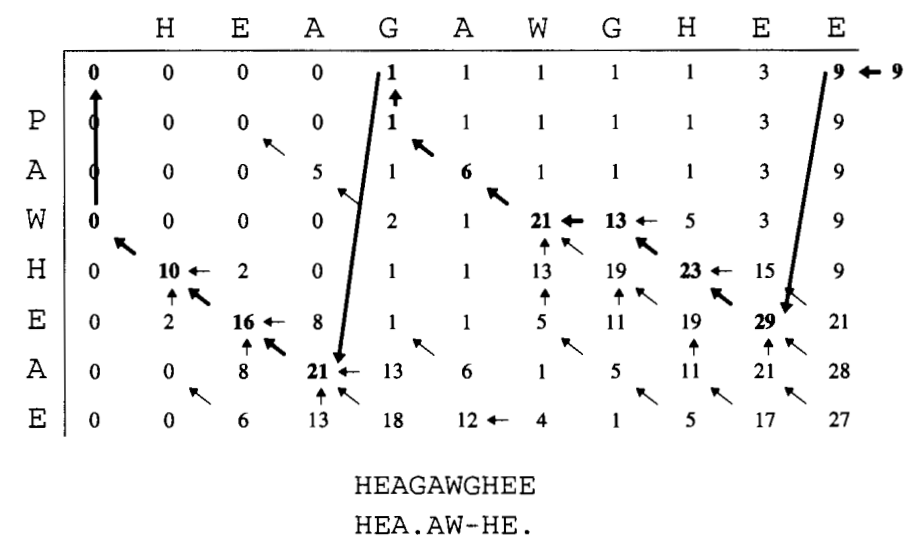
\includegraphics[width=\textwidth]{chapters/approach/smithwatermanrepeated.png}
%	\[
%	\begin{pmatrix}
%                   & - &   & A &   & C &   & A &   &  C & A & C & T & A \\
%	         - & \color{blue}0 & 0 & 0 & 0 & 0 & 0 & 0 & 0 & 0 \\
%	         A & 0 & \color{blue}2 & 1 & 2 & 1 & 2 & 1 & 0 & 2 \\
%	         G & 0 & \color{blue}1 & 1 & 1 & 1 & 1 & 1 & 0 & 1 \\
%	         C & 0 & 0 & \color{blue}3 & 2 & 3 & 2 & 3 & 2 & 1 \\
%	         A & 0 & 2 & 2 & \color{blue}5 & 4 & 5 & 4 & 3 & 4 \\
%	         C & 0 & 1 & 4 & 4 & \color{blue}7 & 6 & 7 & 6 & 5 \\
%	         A & 0 & 2 & 3 & 6 & 6 & \color{blue}9 & 8 & 7 & 8 \\
%	         C & 0 & 1 & 4 & 5 & 8 & 8 & \color{blue}11 & \color{blue}10 & 9 \\
%	         A & 0 & 2 & 3 & 6 & 7 & 10 & 10 & 10& \color{blue}12
%	\end{pmatrix}
%	\]

\subparagraph{Scoring}
Describe how each match is scored

\subparagraph{Match retrival}
	\begin{itemize}
		\item retrieve matches that reach a defined threshold from each alignment pair
		\item Due the nature of this algoritm, all matches that can be found have this minimal score
		\item A match consists of 2 sequences of numbers. 
		\item for each found match:
		\item Search match in all user sessions
		\item From the most to the least found match:
	\end{itemize}
\subsubsection{Model generation}
	\begin{itemize}
		\item Generate Model From Match is done the following way:
		\item For each position of the Match: 
		\item (remind, that each match has 2 Sequences of aligned numbers)
		\begin{itemize}
			\item If Both numbers are equal: The model at this position is the Task refered by this number
			\item If one sequence has a gap at this position: The other EventTask is inserted as an optional
			\item If both numbers differ a selection is inserted. Which kind of selection depends on what the following task is. We don't want to have 2 selections next to each other, instead, create one selection and add each sequence as a sequence
			\begin{itemize}
				\item If the next position also would be a selection, the selection has 2 sequences as a child. those sequences consists of the tasks of each sequence of the match until there is no more selection found 
				\item If the next position is something else we just have a single selection, just add the tasks of the match at this position as childs to the selection
				\item (This description here is really bad, will need some examples)
			\end{itemize}
		\end{itemize}
	\end{itemize}

\subsubsection{Replacement}
	\begin{itemize}
		\item Replace each model in the user sessions
	\end{itemize}

\subsection{Repetition}



